\documentclass[capstone_report.tex]{subfiles}
\begin{document}
\chapter{Requirements gathering and preliminaries}
URSA is a project of significant complexity and open-ended requirements. To manage this, we first detailed the role URSA would play in a crowded landscape of emergency services technologies. We then engaged in the documentation of system requirements, discussion with our key stakeholders, and agreement on the project management tools and techniques which we would use throughout the course of the project.\\

This chapter details our process of preparing requirements and scope, initial engagement with stakeholders, proposed milestones, and agreement on governance and management frameworks. In short, we detail what we planned to achieve, how we planned to achieve it, and timing for when it would be achieved.

\pagebreak

\section{Introduction}
    The metropolitan fire brigade (MFB) provides fire and emergency services to almost three million Melbourne residents in the metropolitan district \cite{MFB_about}.  Although primarily known for dealing with fires, their roles and responsibilities extend to other emergencies including chemical spillages, car crashes, hostage situations and post fire investigations.\\

    A common theme amongst these scenarios is the expectation for firefighters to enter adverse conditions where they have little or no prior knowledge. Examples of this may include; smoke filled environments (low visibility), entering structurally unsound areas, locating and extinguishing small fires, responding to chemical spillages without knowledge of the contents or taming fires that may have toxic smoke.\\

    Under these conditions MFB personnel are required to effectively coordinate their team and make time critical decisions.  The rate at which data can be gathered has tangible outcomes on people's safety and the speed of their response.  In come cases it may not be possible to retrieve the required information to take action (e.g. unknown structural stability), effectively limiting the types of scenarios they can respond to.\\

    As a result the MFB dedicates resources to exploring ways in which it can provide both its on ground personnel and strategists the tools to make the best possible decisions.\\

    One avenue that the MFB has begun exploring is drone technology.  In particular, off the shelf DJI drones \cite{DJI} fitted with thermal cameras (Figure \ref{fig:current_drone}) have been providing the MFB with a birds eye perspective of response scenes.  This use of technology is a significant advantage over traditional ladder platforms that are limited by their observation height and do not carry the required sensors for thermal and plume analysis.

    \begin{figure}  [H]
	\centering
        \includegraphics[width=0.6\linewidth]{example-image-a}
        \captionof{figure}{MFB Drone equipped with thermal imaging}
        \label{fig:current_drone}
    \end{figure}

    During its pilot program, their drones have been successfully deployed in a number emergency situations.  A few examples are given below:
    \begin{enumerate}
        \item \textbf{Coolaroo Recycling Plant}: A recycling plant in Melbourne's Northern suburbs caught fire releasing toxic smoke ultimately resulting in the evacuation of 100 residents.  Figure \ref{fig:coolaroo}  shows the birds eye perspective provided by the drone used to inform strategic decisions.
        \item \textbf{Citylink Truck Accident}: One incident on Melbourne's Citylink saw a truck crash into a brige in a way that part of it was obscured from view (\ref{fig:truck}).  A drone provided images to examine vehicle before removal.
        \item \textbf{Post Fire Investigation}  - Aerial images provide evidence in a coroners report.
    \end{enumerate}

    % Examples of current drone technology usage by the MFB
    \begin{figure*}
        \centering
        \begin{subfigure}[b]{0.33\textwidth}
            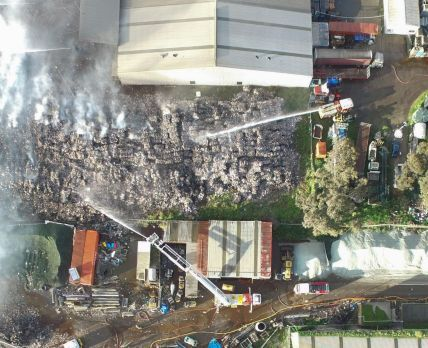
\includegraphics[width=\textwidth]{imgs/coolaroo.jpg}
            \caption{Coolaroo Recycling Plant}
            \label{fig:coolaroo}
        \end{subfigure}
        ~ %add desired spacing between images, e. g. ~, \quad, \qquad, \hfill etc. 
          %(or a blank line to force the subfigure onto a new line)
        \begin{subfigure}[b]{0.33\textwidth}
            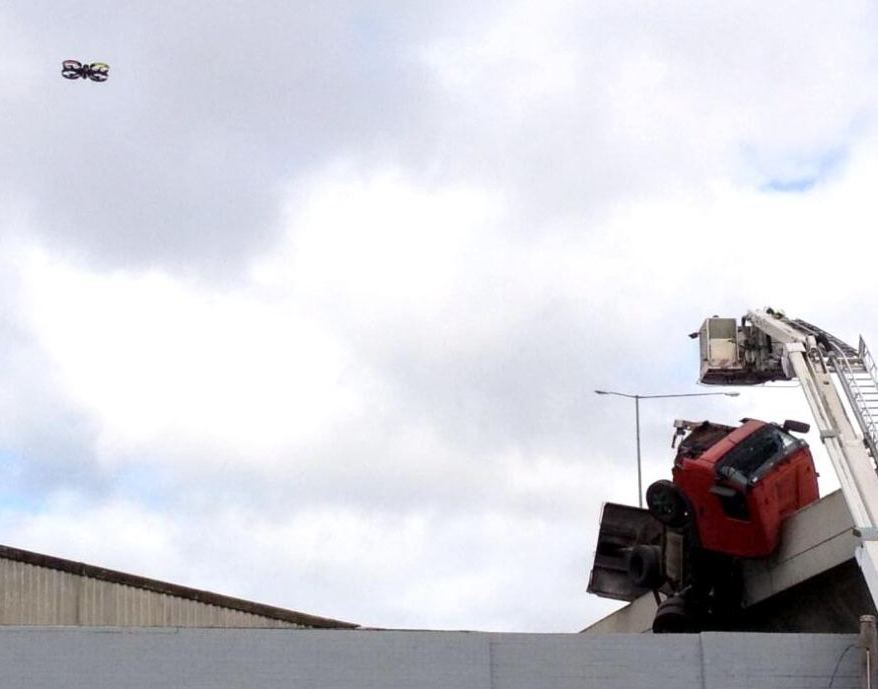
\includegraphics[width=\textwidth]{imgs/truck.jpg}
            \caption{Citylink Truck Accident}
            \label{fig:truck}
        \end{subfigure}\\
        ~ %add desired spacing between images, e. g. ~, \quad, \qquad, \hfill etc. 
        %(or a blank line to force the subfigure onto a new line)

        \begin{subfigure}[b]{0.33\textwidth}
            \includegraphics[width=\textwidth]{example-image-c}
            \caption{Post Fire Investigation}
            \label{fig:post_fire}
        \end{subfigure}
        \caption{Examples of current drone technology usage by the MFB}\label{fig:curren_usage}
    \end{figure*}

    Each of these examples show how drones have offered a critical perspective on emergency situations that may have not been possible via traditional methods or may have been too costly (e.g. helicopters).\\

    All examples given above were outdoors because the current state of the program relies solely on manual operation.  Indoor environments are more challenging for human pilots to navigate as consideration needs to be given to stationary and moving obstacles, tighter constraints on flyable areas (doorways, windows) and obscured line of sight to drone.  In addition, indoor environments impose harsher operating conditions including higher temperatures and limited visibility from smoke.  As a result MFB currently does not have any drones that can operate indoors.\\

    Finding a solution to this current limitation would be a worthwhile pursuit as indoor scenarios make up a considerable portion of emergency situations.  Furthermore there a number of use cases that would provide the MFB with a strategic advantage if implemented:

    \begin{itemize}
        \item Remote imaging of areas not yet deemed safe to enter e.g. structurally unsound post earthquake, hostage situations, identifying chemical labels
        \item Remote imaging to strategists of indoor situation currently occupied by firefighters 
        \item Automated floor plan or 3D mapping generation to improve awareness of unknown environments and aid planning
        \item Augmented map with key information including locations of small heat sources,  positions of any humans inside building,  hazards, thermal/plume analysis
        \item Ability to operate drone outside of line of sight to enable co-location of pilot and strategists who may be kilometres away from scene
    \end{itemize}

    Although the benefits are clear, realizing this goal requires overcoming a number of technical challenges.  To fit these use cases requires the development of an autonomous drone with real time simultaneous location and mapping capabilities, obstacle avoidance algorithms and a communication link reliable through walls and over large distances.
    Thankfully, there are already a number of examples of people using drone technology to achieve these outcomes.\\

    Researchers at Carnegie Mellon \cite{purohit2011sensorfly} successfully used a network of miniature, low cost drones collecting temperature, gas, pressure and ceiling height data to predict the propagation of a fire indoors.  Low cost was a necessary design constraint as it allowed multiple drones to be deployed simultaneously to give good spatial and temporal coverage of an area.  Given this limitation the ability to accurately estimate the position of the aerial vehicles was restricted as this capability is typically provided by a more expensive laser scanner unit.  To rely on cheaper estimation sensors such as an inertial measurement unit (IMU) and range sensors, drones explored their environment by conducting a random walk until within a specified distance of the next drone.  Interpolation was then conducted using inter-drone distance to build the 3D model.  In emergency situations such a model would provide fire-fighters with the ability to monitor the progression of a fire in real-time through a building.\\

    An alternative solution to indoor monitoring of fire has been proposed by Myeong et al. (2017) \cite{myeong2017development} which developed a drone capable of mounting walls.  THe ability to mount walls allows for a larger drone platform capable of carrying heavier laser scanning modules (accurate position estimation) but also the flexibility of passing through doorways vertically.  The team also showed their drone was capable of withstanding temperatures of up to 1000$^\circ C$ for 60 seconds.  It was able to achieve this by wrapping the vehicle in aramid fibre (commonly used in fire-fighters) clothing, insulating electric components with an air buffer and utilizing a thermoelectric cooler (TEC).  These promising results show that producing a drone capable of withstanding the harsh conditions is an achievable goal.\\

    \begin{figure}[H]  
	\centering
        \includegraphics[width=0.6\linewidth]{example-image-a}
        \captionof{figure}{Fire-proof drone}
        \label{fig:fire_proof_drone}
    \end{figure}

    Outside of fire based emergencies a number of studies have also been experimenting with drones in earthquake conditions \cite{kruijff2012rescue}, \cite{michael2012collaborative}.  Nathan et al. (2012)  were able to successfully fuse sensor data from a team of collaborative ground and aerial robots to produce 2D and 3D floor plans of multilevel environments.  From the reconstructions, they were able to identify important features including structural braces and caved walls.  The use of ground robots was a solution to overcome the limited payload and flight time capacity of aerieal robots.\\

    In the commercial space products such as the Elios drone are already available on the market \cite{Elios}.  The Elios makes use of a protective spherical cage to make their drone robust to collisions.  As a result, pilots are now able to fly the drone manually without having to be concerned with the complexity of obstacle avoidance in confined spaces.  This approach eliminates the need for heavy and expensive position estimation sensors and simplifies the product development.\\

    \begin{figure}[H]
	\centering
        \includegraphics[width=0.6\linewidth]{example-image-b}
        \captionof{figure}{Elios collision resilient drone}
        \label{fig:fire_proof_drone}
    \end{figure}

    In light of these studies we see that a number of different approaches have been taken to provide fire-fighters with enhanced awareness of emergency situations.  The proposed use cases appear to be achievable with available technology.  In this project we develop a prototype solution for the MFB to expand their current drone capabilities to indoor areas.  We present the approach we took to developing the drone and results after testing in a laboratory setting.\\

    A number of uses cases were presented above with competing design requirements (as we saw from previous studies).  In the next section we outline the scope our project and the success criteria.


\section{Scope of project}
We were given a very broad remit for improving the state of the art with respect to indoor emergency UAVs. Given such a broad remit, it was important to put parameters around our project and ensure that MFB were comfortable with the direction in which we were taking the research and development.\\

Initially, research into the state of the art of UAV technologies was undertaken to develop a sense of the problem at hand and what can realistically be achieved. After a number of brainstorming sessions, consultation with MFB commander Will Glenn and a visit to MFB headquarters, the scope of the project and its desired outcomes was refined. \\

    \begin{figure}[H]  
	\centering
        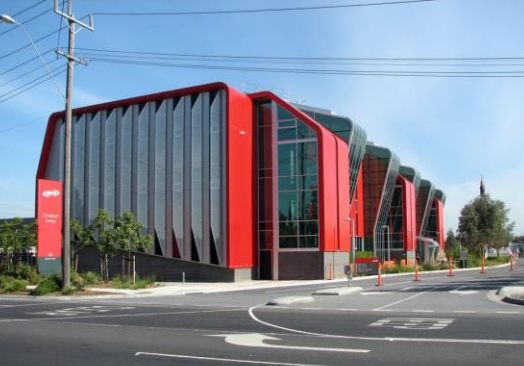
\includegraphics[width=0.6\linewidth]{imgs/mfbBurnley.png}
        \captionof{figure}{MFB Burnley headquarters}
        \label{fig:mfbBurnley}
    \end{figure}

In particular, the following success criteria were proposed:
\begin{itemize}
	\item Autonomous navigation to a destination: Fundamentally, it was required that the drone would operate without control from a pilot and only based on a destination input from a base station. This removes the issues that arise from obscured vision, such as smoke and minimises risk to human health and safety and the drone itself.
	\item Avoidance of obstacles whilst in operation: The drone should be able to avoid collisions with obstacles within an indoor environment, based on sensor readings.
	\item A live image/video feed of an indoors environment: The drone was to obtain vision of the environment, so hazards and fire sources can be spotted.
	\item A live 2D mapping of an indoors environment: To create a visualisation of the layout of the environment so that hazards can be located Initially, 3D mapping was desired but exceeded processing power and memory requirements \footnote{see section on estimation algorithms}.
	\item Safe take-off and landing behaviour: The drone should be able to return to the base station upon completion of its tasks and in the event of low power whilst landing safely. 
\end{itemize}

The above list summarises the main scope of the project. However, for a project as vulnerable to scope creep as URSA, it is almost as important to delineate what is out of scope. On discussion with MFB, it was agree that the features beyond the scope of the project included:
\begin{itemize}
	\item Protection against weathering and dynamic environments: As the drone was to be used as a prototype for future UAV developments, it was decided that environment-proof considerations in real disaster management scenarios, such as the selection of suitable materials, was beyond the scope of this project.
 \item Drone design considerations: An off-the-shelf drone was to be used. In reality, due to our level of customization required, we ended up building the majority of the drone ourselves.
\end{itemize}

Based on this defined scope, we were able to commence the more intricate details of project and deliverable management, which is discussed in the following section.


\section{Project management}
	Since the scope of the project is ambitious, it is crucial to put into place appropriate project planning and project controls in order to ensure success. In particular, this project has budgetary planning requirements, as well as many of the complexities which are inherent to a technical project containing complex hardware and software development tasks. 

\subsection{Budget and BOM}
	The standard capstone project budget is \$130 per student, for a total of \$390. While this is very generous, it is not sufficient for our project. This is because our scope includes building or acquiring a prototype drone. As will be shown in later sections, this cannot be done for less than around \$800. Further, the sensors which we will be required to use are expensive - a typcial entry level LiDAR scanner is over \$1,000. As with the drone, the justifications for these design requirements will be presented in later sections.\\

The conclusion is that additional funding would be required for our project. This was discussed and agreed with our supervisor, and a basic Bill of Materials was prepared. This is attached at Appendix A. The budget for this BOM was \$2,214 in the first instance, plus the use of some additional components already purchased by the University.\\

In addition to this, we were required to purchase incidentals throughout the course of the project. This included heavy gauge wire, 3D printing filament, wiring, connectors and many other minor parts. These incidentals were minor and were able to be absorbed within our allocated student budgets.

\subsection{Project management tools}
	At the outset of the project, we used a number of tools which were taught to us during the project management coursework part of the capstone project. In particular, we generated Gantt charts for the projected tasks, discussed timeframes, and prepared budgets. A simplified timeframe from this phase is outlined below:

\begin{itemize}
\item Construction of the flight platform (April 2017)
\item Programmatic drone flight control (May 2017)
\item Environment mapping (June 2017)
\item Autonomous navigation and photography (August 2017)
\item Extension topics (multi-storey buildings etc) 
\end{itemize}

Of course, good project management is not a case of `set and forget'. During the project, we were also required to revisit this plan and manage tasks to a greater level of detail. For this, we made use of a number of project management tools for planning and tracking of work. Initially, we used a software platform known as Asana to create, allocate and track tasks. Asana uses a Kanban Board based approach, with a sample shown at Figure \ref{fig:asana}. As can be seen, each task is represented by a task, categorised by its progress, and assigned to a person responsible.

    \begin{figure}[H]
	     \centering
	     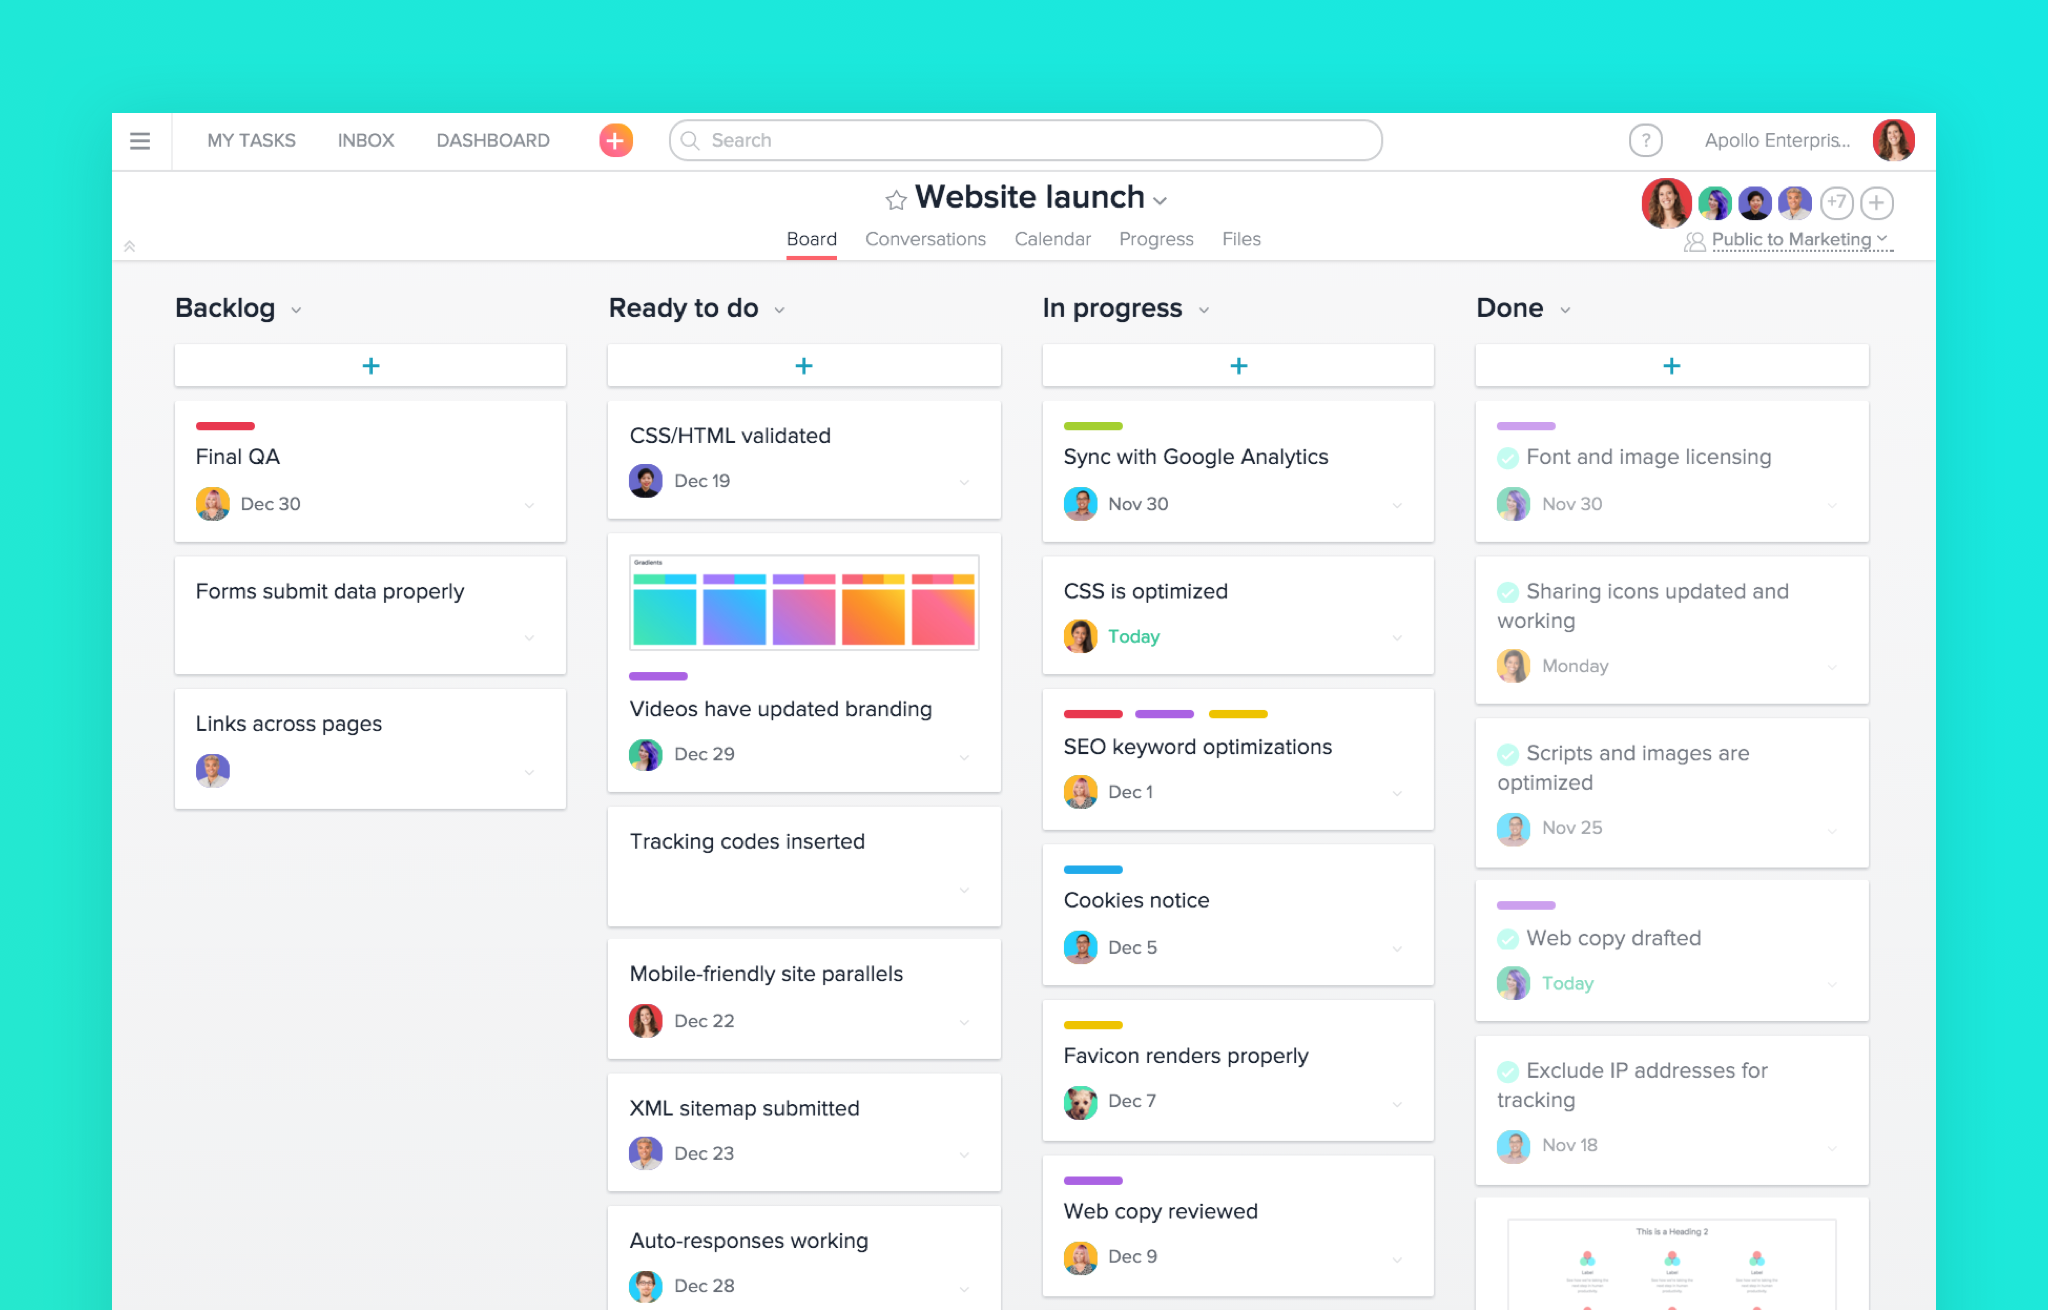
\includegraphics[width=0.8\textwidth]{imgs/asanaBoard.png}
	     \caption{Example of Asana\label{fig:asana}}
	 \end{figure}

Another tool which we used extensively was Git and GitHub. Git is a software version control protocol, whilst GitHub is a web application that allows Git respositories to be hosted online. For our project, we created an `organisation' on GitHub, which can be viewed here: \url{https://github.com/ursa-drone}. The repository naming is fairly self-explanatory when read in conjunction with the remainder of this report. \\

Git was found to be a very powerful tool. We soon found that a large proportion of our project would require complex software development. Git allows branching of versions, making modifications, and then merging those branches back into the master repository. In this way, many users could work on the same code simultaneously, with the only application of thought to synchronisation being required when conflicts between users' code occurred. Even in this case, Git provides powerful tools for conflict resolution.\\

We found our reliance on GitHub grew to the point where its simple issues tracking system was much more convenient to use than Asana's. This was so even though GitHub's issue tracking was incredibly basic and lacked many of the apparently superior features of Asana. The appeal of GitHub was that issues could be linked directly to changes in code, rather than input as an afterthought. We soon migrated all of our task and issue tracking to GitHub. This is an interesting insight into project management and the tools used for managing complex projects - we found that they work best when they are organic, integrated into normal workflow, rather than an additional layer of administration on top of the work already done. Issues tracked in GitHub can be accessed at the following URL: \url{https://github.com/ursa-drone/ursa-server/issues}.\\

Equipped with these tools, and prepared as we were by the capstone project management coursework, we found managing tasks to deliver on-time to be straightforward.

\end{document}